\chapter{State of the Art}

In this chapter we describe the state of the art of recommender systems.\\
In the first section we start from the basic principles of recommender systems, covering the standard techniques, such as content-based, collaborative and hybrid recommender systems. After that, we will cover the matrix factorization model.\\
In the second section we will cover the metrics used to evaluate datasets and recommender systems results.\\
The third sections describes the state of the art of knowledge transfer techniques used in recommender systems.\\
The fourth section describes clustering techniques and their use in recommender systems.



\section{Basic principles of Recommender Systems}

In this section we will start by giving a brief definition of recommender systems and the problems they are faced with.\\
The most accurate definition of modern recommender systems can be found in Burke's statement:\\
"Any system that produces individualized recommendations as output or has the effect of guiding the user in a personalized way to interesting or useful objects in a large space of possible options." (Burke, 2002)


\subsection{Recommender Systems Tasks}

While recommender systems in general are aiming at learning and anticipate user preferences to provide helpful suggestions, they are faced with two distinct tasks: items ranking and items ratings prediction.\\
Ranking is the task of selecting from the whole catalog a small number of items to be recommended for each user. We can distinguish two slightly different scenarios for the ranking task. If an item of the catalog can be interacted with multiple times, every item should be eligible for recommendation. For example, in a music streaming service, users usually listen to the same song several times. On the contrary, if users are not expected to choose the same item twice, already rated or seen items are excluded from the items the recommender systems suggests.\\
Rating prediction consists in providing a computed rating for each user unrated item. Since items with predicted ratings can then be ordered and selected for ranking, most of the times the two tasks share some characteristics, while the main differences between them are identified in the evaluation test set and metrics.


\subsection{Types of Feedback}

Since recommender systems can leverage historical data and user profiles, it is important to distinguish two types of feedback.
Explicit feedback are clear and numerical values of how much a user liked or disliked an item he interacted with.
While explicit feedback is the most accurate indicator of user preferences and, for this reason, it makes the recommendation task easier, they are usually hard to obtain from users, since a user input is required. Additionally, explicit feedback can easily be user biased, as different users could value a numeric rating differently.\\
Implicit feedback is identified as the user interaction with an item. For example, the action of listening to a song on a streaming service is considered implicit feedback.
Implicit feedback cannot differentiate between positive and negative feedback and as such it is always available but considered less reliable than explicit ratings.


\subsection{Data Structures}

Recommender systems often make use of common data structures, which can identified in the following matrices:

\begin{itemize}

\item \textbf{User-Content Matrix (UCM)}: Given a set of users $U$ and a set of user labels $L$, the UCM is a matrix with shape $|U| \times |L|$ where each row represents a user $u \in U$ and each column represents a label $l \in L$. Each cell $(u,l)$ represents the value of label $l$ of the user $u$. It can be a real, integer or binary value depending on the nature of the label. For example, to describe the user age, we could either have a single integer label, where each cell value would represent the age of the user, or multiple binary labels representing different age brackets, where each cell value would be:
\begin{equation}
  (u,l)=
  \begin{cases}
    0, & \text{if}\ u\ \text{belongs to the age bracket}\ l\\
    1, & \text{otherwise}
  \end{cases}
\end{equation}
The approach of splitting a numerical label into multiple categorical labels is called one-hot encoding.\\
The UCM is generally built in content based recommendation approaches.

\item \textbf{Item-Content Matrix (ICM)}: Given a set of items $I$ and a set of item labels $L$, the ICM is a matrix with shape $|I| \times |L|$ where each row represents an item $i \in I$ and each column represents a label $l \in L$. Each cell $(i,l)$ represents the value of label $l$ of the item $i$. It can be a real, integer or binary value depending on the nature of the label.\\
Similarly to the UCM, the ICM is generally built in content based recommendation approaches.

\item \textbf{Similarity Matrix}: Given a set of items $I$, the similarity matrix is a matrix with shape $|I| \times |I|$ where each row $i_r$ and column $i_c$ represent an item $i \in I$ and each cell represent the similarity between $i_r$ and $i_c$. The same structure is used for user similarity.

\item \textbf{User-Rating Matrix (URM)}: Given a set of users $U$ and a set of items $I$, the URM is a matrix with shape $|U| \times |I|$ where each row represents a user $i \in I$ and each column represents an item $i \in I$. Each cell $(u,i)$ represents the value of the rating of the item $i$ by user $u$. It can be a real, integer or binary value depending on the nature of the feedback. For example, in the scenario of explicit feedback, each cell would have a real or integer value, usually with upper and lower bounds, while in the scenario of an implicit feedback, each cell value would be:\\
\begin{equation}
  (u,l)=
  \begin{cases}
    0, & \text{if}\ u\ \text{interacted with item}\ i\\
    1, & \text{otherwise}
  \end{cases}
\end{equation}
The URM is generally built in collaborative filtering recommendation approaches.

\end{itemize}


\subsection{Similarities}

A similarity function is mathematical tool to compute the similarity between two entities represented in a space, as a numerical value. In the field of recommender systems similarity functions are often used to extract similar entities from a dataset, given a target user or item. It is then important to mention and describe the commonly used ones.

\begin{itemize}

\item \textbf{Cosine similarity}: given two vectors $x$ and $y$, the cosine similarity is computed as follows:
\[ S_{xy} = \frac{x \times y}{||x||\||y|| + h} \]
where $h$ is the shrink term for normalization.
This similarity measures the angle between n-dimensional vectors. Since the angle can vary between 1 and -1, $S_{xy} \in [-1, 1]$. If $S_{xy} = 1$ we have complete similarity (parallel vectors); if $S_{xy} = 0$, we have no similarity (orthogonal vectors) and if $S_{xy} = -1$ we have inverse similarity (parallel vectors with inverse direction).\\
The cosine similarity is between the two most popular similarities used in recommender systems.

\item \textbf{Pearson correlation}: given two random variables $X$ and $Y$, the Pearson correlation can be computed as follows:
\[ \rho_{X,Y} = \frac{cov(X,Y)}{\sigma_x \sigma_y} \]
where $cov(X,Y)$ is the covariance between $X$ and $Y$ and $\sigma_x$ and $\sigma_y$ are respectively the standard deviations of $X$ and $Y$.\\
Since we need to apply the formula to a sample, we can give the following definition. Given two vectors $x$ and $y$ of dimension $n$, the pearson correlation is computed as follows:
\[ S_{xy} = \frac{\sum_{i}^{n} (x_i - \bar{x})(y_i - \bar{y})}{\sqrt{\sum_{i}^{n} (x_i - \bar{x})^2}\sqrt{\sum_{i}^{n} (y_i - \bar{y})^2} + h} \]
where $\bar{x}$ and $\bar{y}$ are respectively the means of $x$ and $y$ and $h$ is the shrink term for normalization.\\
Like with the cosine similarity $S_{xy} \in [-1, 1]$, where -1 means positive linear correlation, 0 means no linear correlation and -1 means negative linear correlation. It is very popular in recommender systems.

\item \textbf{Jaccard coefficient}: given two vectors $x$ and $y$, the Jaccard coefficient is computed as follows:
\[ S_{xy} = \frac{x \times y}{|x| + |y| - xy + h} \]
where $h$ is the shrink term for normalization.\\
The Jaccard coefficient is ranged in the interval $[0, 1]$ and is used to compute the similarity between two finite sets and can be applied with binary values.

\item \textbf{Dice coefficient}: given two vectors $x$ and $y$, the Dice coefficient is computed as follows:
\[ S_{xy} = \frac{x \times y}{\frac{1}{2}|x| + \frac{1}{2}|y| - xy + h} \]
where $h$ is the shrink term for normalization.\\
It ranges in the interval $[0, 1]$ and, like the Jaccard coefficient, it is used to compute the similarity between finite sets and can be applied with binary values.

\item \textbf{Tanimoto coefficient}: given two vectors $x$ and $y$ of dimension $n$, the Tanimoto coefficient is computed as follows:
\[ S_{xy} = \frac{\sum_{i = 1}^{n} x_iy_i}{\sum_{i = 1}^{n} x_i^2 + \sum_{i = 1}^{n} y_i^2 - \sum_{i = 1}^{n} x_iy_i} \]
where $h$ is the shrink term for normalization.\\
It ranges in the interval $[0, 1]$ and, like Jaccard and Dice coefficients, it is used to compute the similarity between finite sets and can be applied with binary values.

\end{itemize}



\section{Types of Recommender Systems}

There exist several types of recommender systems, but they can mainly be divided into three macro-types.


\subsection{Content-based Filtering (CBF)}

When users or items characteristics are available, it is possible to leverage them to create personalized recommendations. For example, clothing digital stores may use colors of clothing as a label to compute items similarity. The objective of this type of recommender systems is to use one or more labels for each user or item, starting from their characteristics, and exploit them to identify similar entities. We can distinguish between item-based and user-based CBF.

\begin{itemize}

\item \textbf{Item-based}: given the set of items $I$ and the set of users $U$, for each user $u \in U$ we define $I_u$ as the set of items rated by user $u$. To recommend items to user $u$, the system exploits the ICM to compute the similarities between each item $i_u \in I_u$ and $i \in I$ by building an item similarity matrix with shape $|I_u| \times |I|$.\\
Then, it computes the estimated rating of each item $i$ by user $u$ as follows:
\[ \hat{r}_{ui} = \frac{\sum_{i_u \in I_u} r_{ui_u} * ISIM_{i_u,i}}{\sum_{i_u \in I_u} ISIM_{i_u,i}} \]
where $r_{ui_u}$ is the rating of item $i_u$ by user $u$ and $ISIM$ is the item similarity matrix. The normalization is useful to compute accurate ratings, but can be left out for top-n recommendation.\\
Items with the highest ratings, excluding items in $I_u$, are recommended to user $u$.
To avoid computing the similarity matrix for each user, it is possible to build a single item similarity matrix with shape $|I| \times |I|$ and consider, for each user, only the items contained in $I_u$.

\item \textbf{User-based}: given the set of items $I$ and the set of users $U$, for each user $u \in U$ we define $I_u$ as the set of items rated by user $u$. Similarly to the item-based approach, a user similarity matrix with shape $|U| \times |U|$ is built starting from the UCM.\\
The estimated rating of each item $i \in I$ by user $u$ is computed as follows:
\[ \hat{r}_{ui} = \frac{\sum_{v \in U} r_{vi_u} * USIM_{u,v}}{\sum_{v \in U} USIM_{u,v}} \]
Items with the highest ratings, excluding items in $I_u$, are recommended to user $u$.

\end{itemize}

The main advantage of CBF is that it makes possible to solve the cold start problem, both for users and items, when their features are available. By leveraging the users and items features to provide recommendations, CBF bypasses the problem completely.


\subsection{Memory-based Collaborative Filtering}

Memory-based collaborative filtering recommender systems exploit the assumption that similar users will likely prefer the same items. They use interactions as a bridge to identify similar users or items, called neighbors. The goal of this approach is then to compute a neighborhood for target users or items. In order to describe the methodology, we must distinguish between user-based and item-based.

\begin{itemize}

\item \textbf{User-based}: in the user-based approach, the goal of the system is to compute a neighborhood for the user $u$ needing recommendations. This is defined as the set of users similar to $u$ based on their preferences. Their own preferences are then used to extract recommendation for the user $u$.\\
Given the set of users $U$ and the set of items $I$, the system exploits the URM to build a user similarity matrix with shape $|U| \times |U|$.\\
We define $URM_u$ as the set of items rated by user $u$ and $URM_{u,i}$ as the rating of item $i$ by user $u$.\\
The estimated rating of each item $i \in I$ by user $u$ is computed as follows:
\[ \hat{r}_{ui} = \frac{\sum_{v \in U \wedge v \neq u} URM_{v,i} * USIM_{u,v}}{\sum_{v \in U} USIM_{u,v}} \]
Items with the highest ratings, excluding items in $URM_u$, are recommended to user $u$.

\item \textbf{Item-based}: the item-based approach is slightly different. In this scenario, the system computes the neighborhood of the item $i$ and then recommends it to users belonging to the neighborhood that are yet to interact with it.\\
Given the set of users $U$ and the set of items $I$, the system exploits the URM to build an item similarity matrix with shape $|I| \times |I|$.\\
Like in the user-based approach, we define $URM_u$ as the set of items rated by user $u$ and $URM_{u,i}$ as the rating of item $i$ by user $u$.\\
The estimated rating of each item $i \in I$ by user $u$ is computed as follows:
\[ \hat{r}_{ui} = \frac{\sum_{j \in I \wedge j \neq i} URM_{u,j} * USIM_{i,j}}{\sum_{j \in I} USIM_{i,j}} \]
Items with the highest ratings, excluding items in $URM_u$, are recommended to user $u$.

\end{itemize}


\subsection{Model-based Collaborative Filtering}

Model-based collaborative filtering recommender systems exploit the URM with a machine learning model to provide recommendations. There are many different ways to do so and in this thesis we will cover matrix factorization in \autoref{matrix-factorization} and factorization machines in \autoref{factorization-machines}.


\subsection{Hybrid}

Different recommender systems have different strengths and weaknesses. Many different types of hybrid systems have been developed to overcome the weaknesses of the single approaches. There are multiple techniques that can be used to combine the results. The most common technique is to combine the items scores into a single recommendations by assigning weights. Alternatives are switching recommender system based on the scenario or to use different systems in cascade to refine previous recommendations.



\section{Matrix Factorization}
\label{matrix-factorization}

Matrix factorization \cite{10.1109/MC.2009.263} is a way of computing matrix decomposition: reducing a matrix into the product of two other matrices. After winning the Netflix Prize competition in 2009, it became a very popular approach in recommender systems.\par
The assumption of matrix factorization is that it is possible to extract latent factors, to characterize users and items, from the rating pattern. For items, these factors represent an alternative to the human generated features. For users, the factors represent how much a user prefers items with a high score in the corresponding factor. For this reason, we say that matrix factorization is an approach for latent factors models.\par
Given a set of users $U$ and a set of items $I$, matrix factorization models decompose the URM so that users and items are mapped to a latent factor space of dimensionality $f$ and their interactions are modeled as inner products in that space. Each user $u \in U$ is associated with a vector $p_u \in \mathbb{R}^f$ and each item $i \in I$ is associated with a vector $q_i \in \mathbb{R}^f$.\\
For each user $u$, the values of $p_u$ measure how much the user likes items characterized by the corresponding factor. For each item $i$, the values of $q_i$ measure how much the item is characterized by that factor.\\
The estimated rating of item $i$ by user $u$ is then computed as follows:
\[ \hat{r}_{ui} = q_i^T p_u \]\par
The challenge of matrix factorization is building the mappings for users and items.


\subsection{Stochastic Gradient Descent (SGD)}

SGD is a popular approach \cite{ImprovingSVD, 10.1145/1401890.1401944, 10.1145/1345448.1345466} to compute the latent factors mappings. It involves cycling all the training ratings and computing the error:
\[ e_{ui} = r_{ui} - q_i^T p_u \]
Then, the values are modified by a magnitude proportional to $\gamma$ in the opposite direction of the gradient, as follows:
\begin{equation*}
\begin{split}
& p_u \gets p_u + \gamma (e_{ui} q_i - \lambda p_u) \\
& q_i \gets q_i + \gamma (e_{ui} p_u - \lambda q_i)
\end{split}
\end{equation*}
where the costant $\lambda$ determines the extent of regularization.



\section{Factorization Machines (FM)}
\label{factorization-machines}

Factorization machines \cite{10.1109/ICDM.2010.127} are a relatively new technique of collaborative filtering with side information proposed by Steffen Rendle in 2010. Since they are a general-purpose supervised learning algorithm, they can be adapted to work with recommender systems.\\
Given $S$ the set of tuples $(\bar{x}, y)$ where $\bar{x} = (x_1, ..., x_k) \in \mathbb{R}^k$ is a k-dimensional feature vector and $y$ is the corresponding class label, using factorized interactions, FM models all possible interactions between variables in $\bar{x}$.\\
The FM model equation is defined as follows:
\begin{equation*}
\hat{y}(\bar{x}) = w_0 + \sum_{i = 1}^{n} w_i x_i + \sum_{i = 1}^{n} \sum_{j = i + 1}^{n} \langle v_i, v_j \rangle x_i x_j
\end{equation*}
where $w_0 \in \mathbb{R}$ is the global bias, $w_i \in \mathbb{R}$ is the bias of feature $i$, vector $v_i \in \mathbb{R} \times f$ is the interaction parameter vector of feature $i$ and $\langle \cdot, \cdot \rangle$ is the dot product of two vectors of size k:
\begin{equation*}
\langle v_i, v_j \rangle = \sum_{f = 1}^{k} v_{i,f} \cdot v_{j,f}
\end{equation*}



\section{Dataset Metrics}

The main characteristic of a dataset is sparsity. Given a user rating matrix, sparsity is the ratio of observed to total ratings. %(https://arxiv.org/pdf/1205.3193.pdf)



\section{Evaluation Metrics}

When designing or evaluating a recommender system, metrics a fundamental point to understand and use correctly. Depending on the characteristics that need to be evaluated, different sets of metrics have different meanings.


\subsection{Accuracy metrics}

Accuracy metrics are meant to evaluate ranking. They measure the predictiveness of the recommender system; how good its decisions are. The most popular accuracy metrics are Mean Average Precision (mAP) and Normalized Discounted Cumulative Gain (nDCG). Both of them evaluate how good the recommender is to put the most relevant items first in the recommendation list.\par
mAP is outfitted with a top-n threshold which defines how many recommended items are considered for the metric computation. mAP@n is then used to indicate mAP computed on the first n items recommended to each user.\\
We define Precision of the query for user $i$ as
\[ P@k_i = \frac{relevant\_items@k_i}{k} \]
Where $relevant\_items@k$ is the amount of relevant items included in the recommendations list up to rank $k$.\\
We then define Average Precision of the query for user $i$ as
\[ AP@n_i = \frac{1}{TP} \sum_{k=1}^{n} (P@k_i * rel@k) \]
where $TP$ is the total amount of ground truth items and $rel@k$ equals 1 if the item at rank k is relevant and equals to 0 otherwise.\\
Finally, mAP is defined as
\[ mAP@n = \frac{1}{U} \sum_{i=1}^{U} AP@n_i \]
where $U$ is the amount of users.\par
Like mAP, nDCG is computed with a top-n threshold.\\
We define Cumulative Gain as
\[ CG@n = \sum_{k=1}^{n} rating@k \]
where $rating@k$ is the predicted rating of the item at rank $k$.\\
Discounted Cumulative Gain is then computed to penalize ratings based on their position
\[ DCG@n = \sum_{k=1}^{n} \frac{rating@k}{\log(i+1)} \]
Then the result is normalized to make it irrelevant of the query. To do so, we compute the Ideal DCG
\[ IDCG@n = \sum_{k=1}^{|REL_n|} \frac{rating@k}{\log(i+1)} \]
where $REL_p$ is the list of relevant items up to position $n$.\\
Finally, nDCG is defined as
\[ nDCG@n = \frac{DCG@n}{IDCG@n} \]


\subsection{Error metrics}

Error metrics are used to compare actual and predicted ratings, thus are generally used for rating prediction. The most commonly used error metrics are Mean Absolute Error (MAE) and Root Mean Squared Error (RMSE).
MAE is defined as
\[ MAE = \frac{1}{U*I} \sum_{u=1}^{U} \sum_{i=1}^{I} |r_{u,i} - \hat{r}_{u,i}| \]
where $U$ is the amount of users, $I$ is the amount of items, $r_{u,i}$ is the predicted rating of item $i$ by user $u$ and $r_{u,i}$ is the true rating of item $i$ by user $u$.\\
As the formula suggests, MAE does not apply a different weight to outliers, large error values.\par
To compute a weighted error, we define RMSE as
\[ RMSE = \sqrt{\frac{1}{U*I} \sum_{u=1}^{U} \sum_{i=1}^{I} (r_{u,i} - \hat{r}_{u,i})^2} \]


\subsection{Diversity}

Gini index, or Gini coefficient, is a well known statistical metric used to measure income inequality. It can be slightly changed in and used in the field of recommender systems to evaluate a system diversity. We call the variation, where higher values mean higher diversity, Gini diversity \cite{Diversity}.\\
It is computed as follows:
\[ gini\_diversity = 2 \sum_{i=1}^{n} \frac{(n + 1 - i) * x_i}{(n + 1) * \sum_{i=1}^{n} x_i} \]
where $n$ is the amount of items and $x_i$ is the numbers of times item $i$ has been recommended.



\section{Clustering Techniques}

Clustering is the operation of grouping similar unclassified elements together according to some properties or features. It is used in many fields of machine learning with different applications and implementations. In this section we cover the main clustering algorithms used in recommender systems, paying particular attention to the one used in this thesis.


\subsection{K-Means Clustering}

K-Means clustering is the most used and well-known iterative clustering algorithm.\\
To apply K-Means clustering it is necessary to define the number of target clusters. For each cluster, a centroid with random coordinates is initialized.
\begin{itemize}
\item Each element is classified by computing the euclidean distance between its position in space and each centroid. The element is assigned to closest centroid.
\item The centroid is moved by computing the mean of the distances between it and all the elements assigned to it.
\item The process is repeated until the the centroid are only slightly moved or until a maximum amount of iterations is reached.
\end{itemize}
\begin{figure}[htbp]
	\begin{center}
		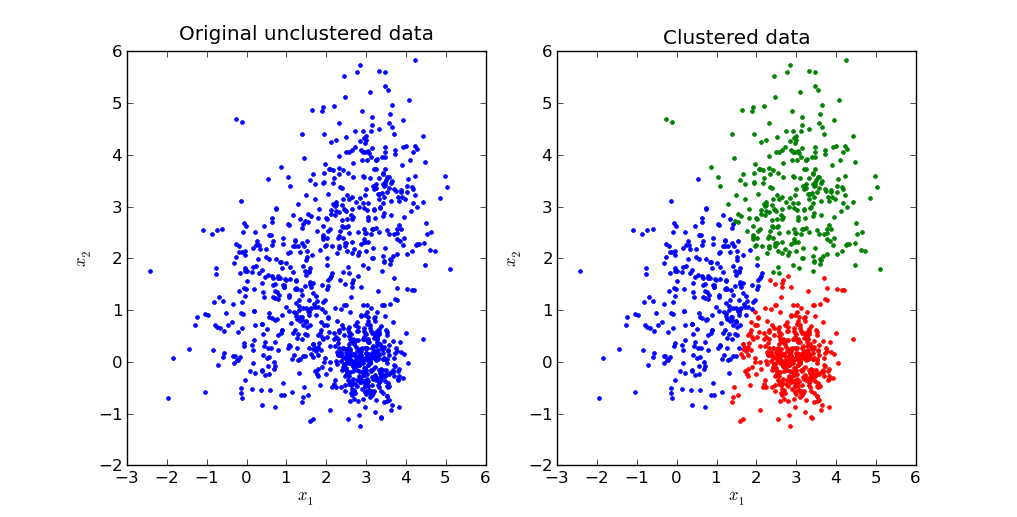
\includegraphics[width=\textwidth]{pictures/k-means-clustering}
		\caption{Results of the K-Means clustering algorithm. Source: https://i.stack.imgur.com/cIDB3.png}
	\end{center}
\end{figure}
K-Means clustering has linear complexity $O(n)$, thus it is considered a fast clustering algorithm.


\subsection{Non-Negative Matrix Factorization (NMF)}

Non-Negative matrix factorization is a set of algorithms for high dimensional data analysis that extracts features from a set of non-negative vectors. It was first introduced by an article by Paatero and Tapper in 1994 \cite{10.1002/env.3170050203} and has been widely used ever since it was made popular by Lee and Seung in 1999 \cite{10.1038/44565}, with the first simple algorithm.\\
It has been proved empirically by different experiments \cite{10.5555/1005332.1044709, 10.1109/CVPR.2001.990477} that NMF has clustering effects.
Given a metrix $X$ with shape $m \times n$, the goal of NMF is to compute matrices $F$, with shape $m \times p$, and $G$, with shape $p \times n$, such that:
\begin{equation*}
X = FG
\end{equation*}
by solving the optimization problem:
\begin{equation*}
\min_{F \in \mathbb{R}^{m \times p}_+, G \in \mathbb{R}^{p \times n}_+} ||X - FG||^2_F
\end{equation*}
where $||X - FG||^2_F$ is the Frobenius norm, defined as:
\begin{equation*}
||X - FG||^2_F = \sum_{i,j} (X - FG)^2_{i,j}
\end{equation*}
The standard NMF algorithm is the following:
\vskip 0.7cm
\begin{algorithm}[H]
\SetKwInOut{Input}{Input}
\SetKwInOut{Output}{Output}
\Input{Non-negative matrix $X \in \mathbb{R}^{m \times n}_+$ and factorization rank $r$.}
\Output{$(F,G) \geq 0$ : A rank-$r$ NMF of $X \approx FG$.}
Generate initial matrices $F^{(0)} \geq 0$, $G^{(0)} \geq 0$\;
\For{$t \gets 1$ \KwTo $max\_iteration$}{
  $G^{(t)} \gets G^{(t - 1)} \odot \frac{(F^{(t - 1)})^T X}{(F^{(t - 1)})^T F^{(t - 1)} G^{(t - 1)}}$\;
  $F^{(t)} \gets F^{(t - 1)} \odot \frac{X (G^{(t)})^T}{F^{(t - 1)} G^{(t)} (G^{(t)})^T}$\;
}
\caption{The standard algorithm for NMF}
\end{algorithm}
\vskip 0.7cm
$F$ and $G$ can be initialized randomly or using some other clustering method, such as K-Means clustering.


\subsection{Orthogonal Non-Negative Matrix Tri-Factorizations (ONMTF)}

Orthogonal non-negative matrix factorizations (ONMF) is a type of NMF that, given a metrix $X$ with shape $m \times n$, computes matrices $F$, with shape $m \times p$, and $G$, with shape $n \times p$, such that:
\begin{equation*}
X = FG^T
\end{equation*}
by solving the optimization problem:
\begin{equation*}
\min_{F \in \mathbb{R}^{m \times p}_+, G \in \mathbb{R}^{p \times n}_+} ||X - FG^T||^2_F, \quad \text{s.t.} \quad F^TF = I
\end{equation*}
Alternatively, for the $G$-orthogonal problem is:
\begin{equation*}
\min_{F \in \mathbb{R}^{m \times p}_+, G \in \mathbb{R}^{p \times n}_+} ||X - FG^T||^2_F, \quad \text{s.t.} \quad G^TG = I
\end{equation*}
The algorithms for ONMF are the following:
\vskip 0.7cm
\begin{algorithm}[H]
\SetKwInOut{Input}{Input}
\SetKwInOut{Output}{Output}
\Input{Non-negative matrix $X \in \mathbb{R}^{m \times n}_+$ and factorization rank $r$.}
\Output{$(F,G) \geq 0$ : A rank-$r$ NMF of $X \approx FG^T$.}
Generate initial matrices $F^{(0)} \geq 0$, $G^{(0)} \geq 0$\;
\For{$t \gets 1$ \KwTo $max\_iteration$}{
  $G^{(t)} \gets G^{(t - 1)} \odot \frac{X^T F^{(t - 1)}}{G^{(t - 1)} (F^{(t - 1)})^T F^{(t - 1)}}$\;
  $F^{(t)} \gets F^{(t - 1)} \odot \sqrt{\frac{X G^{(t)}}{F^{(t - 1)} (F^{(t - 1)})^T X G^{(t)}}}$\;
}
\caption{The algorithm for $F$-orthogonal ONMF}
\end{algorithm}
\vskip 0.7cm
\begin{algorithm}[H]
\SetKwInOut{Input}{Input}
\SetKwInOut{Output}{Output}
\Input{Non-negative matrix $X \in \mathbb{R}^{m \times n}_+$ and factorization rank $r$.}
\Output{$(F,G) \geq 0$ : A rank-$r$ NMF of $X \approx FG^T$.}
Generate initial matrices $F^{(0)} \geq 0$, $G^{(0)} \geq 0$\;
\For{$t \gets 1$ \KwTo $max\_iteration$}{
  $G^{(t)} \gets G^{(t - 1)} \odot \sqrt{\frac{X^T F^{(t - 1)}}{G^{(t - 1)} (G^{(t - 1)})^T X^T F^{(t - 1)}}}$\;
  $F^{(t)} \gets F^{(t - 1)} \odot \frac{X (G^{(t)})^T}{F^{(t - 1)} (G^{(t)})^T G^{(t)}}$\;
}
\caption{The algorithm for $G$-orthogonal ONMF}
\end{algorithm}
\vskip 0.7cm
The tri-factorizations \cite{10.1145/1150402.1150420} variant uses three factors instead of two, in the form:
\begin{equation*}
X = FSG^T
\end{equation*}
The optimization problem is the following:
\begin{equation*}
\min_{F \in \mathbb{R}^{m \times p}_+, G \in \mathbb{R}^{p \times n}_+, S \in \mathbb{R}^{p \times r}_+} ||X - FG||^2_F, \quad \text{s.t.} \quad F^TF = I, G^TG = I
\end{equation*}
According to Ding \textit{et al} \cite{10.1145/1150402.1150420}, tri-factorization is capable of clustering rows and columns of the input matrix simultaneously.\\
The rules for updating $F$, $G$ and $S$, are according to the following algorithm:
\vskip 0.7cm
\begin{algorithm}[H]
\SetKwInOut{Input}{Input}
\SetKwInOut{Output}{Output}
\Input{Non-negative matrix $X \in \mathbb{R}^{m \times n}_+$ and factorization rank $r$.}
\Output{$(F,G,S) \geq 0$ : A rank-$r$ NMF of $X \approx FSG^T$.}
Generate initial matrices $F^{(0)} \geq 0$, $G^{(0)} \geq 0$, $S^{(0)} \geq 0$\;
\For{$t \gets 1$ \KwTo $max\_iteration$}{
  $G^{(t)} \gets G^{(t - 1)} \odot \sqrt{\frac{X^T F^{(t - 1)} S^{(t - 1)}}{G^{(t - 1)} (G^{(t - 1)})^T X^T F^{(t - 1)} S^{(t - 1)}}}$\;
  $F^{(t)} \gets F^{(t - 1)} \odot \sqrt{\frac{X G^{(t)} (S^{(t - 1)})^T}{F^{(t - 1)} (F^{(t - 1)})^T X G^{(t)} (S^{(t - 1)})^T}}$\;
  $S^{(t)} \gets F^{(t - 1)} \odot \sqrt{\frac{(F^{(t)})^T X G^{(t)}}{(F^{(t)})^T F^{(t)} S^{(t - 1)} (G^{(t)})^T G^{(t)}}}$\;
}
\caption{The algorithm for ONMTF}
\end{algorithm}



\section{Cross-Domain Recommender Systems}

While the majority of recommender systems provide recommendation targeted only to a single topic, in recent years large digital service companies like Amazon or Google started providing recommendation across a very eterogeneous set of services. Amazon, for example, provides recommendations both for its e-commerce website, for items of all categories, and for music, movies and so on. In this scenario it may be useful to provide recommendation across different domains.\\
Cross-domain recommender systems aim to generate higher quality recommendations in a target domain by leveraging data coming from one more different source domains. In particular, knowledge acquired in a source domain can be transferred with some knowledge-transfer technique to the target domain.\\
The use cases for such approach are mainly two. First, building a user profile across domains allows to generate bundle recommendation \cite{10.1007/s11257-012-9131-2, 10.1007/s11257-007-9042-9, 10.1007/s11257-012-9128-x}. For example it may be possible to recommend the movie transposition of a book the user bought and then to recommend the movie soundtrack. A recommendation like that can only be inferred by exploiting data from multiple domains. The second scenario is the one of the cold start problem \cite{10.1145/2645710.2645777, 10.1007/978-3-642-22362-4_26, 10.1145/2507157.2507206}. Auxiliary source domain may be able information which is missing in the target domain. Both of these scenarios assume that there are correspondences between user and item profiles across domains.\par
A complete review of recommender systems was given by Cremonesi \textit{et al} \cite{10.1007/978-1-4899-7637-6_27}. To introduce their properties and categories we mainly follow their formalization of the problem.


\subsection{Domain Definitions}

The first step in introducting cross-domain recommender systems, is defining the concept of domain. We can distinguish four different levels of domain definition:

\begin{itemize}
\item \textbf{Attribute level}: Two items are considered to belong to different domains if they differ in some attribute. For example two books could be considered of different domains if the differ by genre. The attribute level definition is too weak to be considered for cross-domain recommender systems.
\item \textbf{Type level}: Two items are considered to belong to different domains if they share some attributes but differ by others. For example, TV series and movies belong to different domains, according to this definition.
\item \textbf{Item level}: Two items are considered to belong to different domains if they don't share any attribute, or at least very few. For example, movies and books belong to different domains, according to this definition.
\item \textbf{System level}: Two items are considered to belong to different domains if they belong to different systems, even if they share the same attributes. For example, movies from the Netflix system and movies from the Amazon system belong to different domains, according to this definition.
\end{itemize}


\subsection{Types of recommendation}

The goal of cross-domain recommender systems can also vary depending on which domain is the target for recommendations.\\
According to Cremonesi \textit{et al} \cite{10.1007/978-1-4899-7637-6_27}, we can distinguish three types of recommendations. Given the target domain $D_T$ with its users and items sets, respectively $U_T$ and $I_T$, and one or more source domains $D_S$ with their users and items sets, respectively $U_S$ and $I_S$, we distinguish the following types or recommendation types:
\begin{itemize}
\item \textbf{Multi-domain recommendation}: recommend items in $I_S \cup I_T$ to users in $U_S$ or to users in $U_T$. This approach requires a significant amount of users overlap between domains, but it is becoming feasible due to the amount of profiles maintained by users on different social media, connected by mechanisms of cross-authentication and identification \cite{10.1016/j.ins.2008.08.022} or interoperability \cite{10.1007/s11257-011-9097-5}.
\item \textbf{Linked-domain recommendation}: recommend items in $I_T$ to users in $U_S$ or $U_T$ by exploiting knowledge about $U_S \cup U_T$ and $I_S \cup I_T$. This approach is used to enrich data in a target domain with a cold start or data sparsity problem. Generally, it requires at least a partial amount of users or items overlap between the source and target domains.
\item \textbf{Cross-domain recommendation}: recommend items in $I_T$ to users in $U_S$ or $U_T$ by exploiting knowledge about $U_S$ and $I_S$. This approach is used when the target domain has no information about the users. In this scenario there is no assumption of data overlap between domains and the approaches aim at transferring knowledge from one domain to the other.
\end{itemize}


\subsection{Types of Overlap}

We can then make distinction between four types of overlap:
\begin{itemize}
\item \textbf{No overlap}: Neither the user nor the item sets share common data, such that:
\begin{equation*}
U_T \cap U_S = \emptyset \quad \text{and} \quad I_T \cap I_S = \emptyset
\end{equation*}
\item \textbf{User overlap}: Only the user sets share common data, such that:
\begin{equation*}
U_T \cap U_S \neq \emptyset \quad \text{and} \quad I_T \cap I_S = \emptyset
\end{equation*}
\item \textbf{Item overlap}: Only the item sets share common data, such that:
\begin{equation*}
U_T \cap U_S = \emptyset \quad \text{and} \quad I_T \cap I_S \neq \emptyset
\end{equation*}
\item \textbf{User and item overlap}: Both user and item sets share common data, such that:
\begin{equation*}
U_T \cap U_S \neq \emptyset \quad \text{and} \quad I_T \cap I_S \neq \emptyset
\end{equation*}
\end{itemize}

\begin{figure}[hbt!]
  \centering
  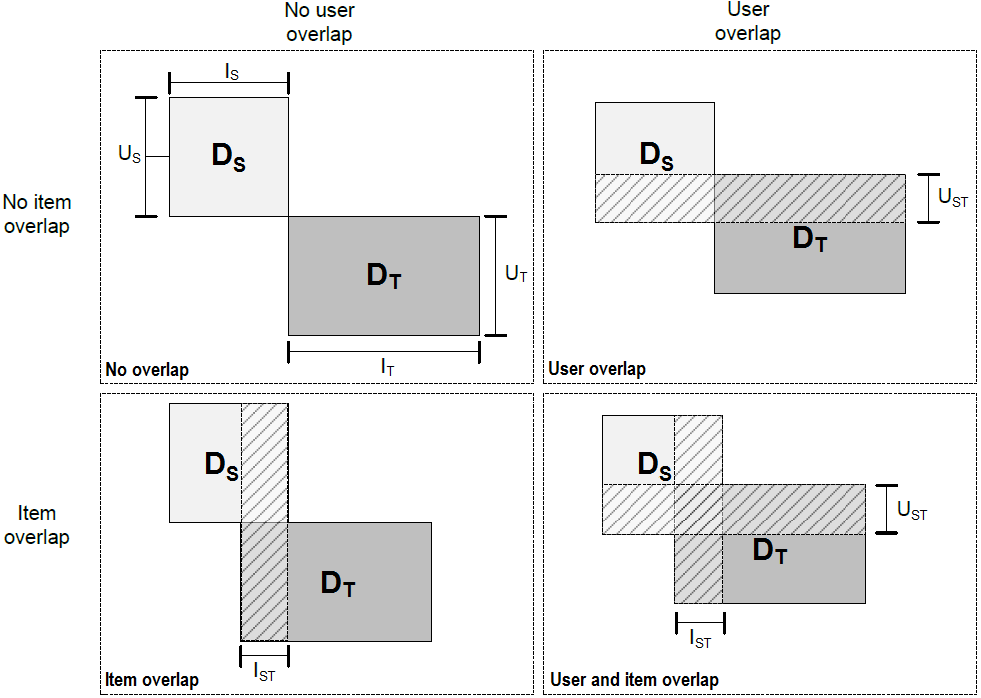
\includegraphics[width=\textwidth]{pictures/domains-overlap}
  \caption{Types of overlap of user and item sets between two domains. Source: https://doi.org/10.1007/978-1-4899-7637-6\_27}
\end{figure}


\subsection{Systems Categories}

Given the previous attributes, different cross-domain recommender system trends have been defined into a categorization by Loizou \cite{crossdomain-recsys-categorization}, which was later enhanced by Cremonesi \textit{et al} \cite{crossdomain-recsys-categorization} into four groups:

\begin{itemize}
\item As proposed by Lee \cite{10.1016/S0957-41740100034-3}, extract association rules from rating behavior in source domains, to be used in the target domain.
\item As proposed by Cao \textit{et al.} \cite{10.5555/3104322.3104344} and Zhang \textit{et al.} \cite{10.5555/3023549.3023635}, learn inter-domain similarity based on ratings and correlation matrices.
\item As proposed by Zhuang \textit{et al.} \cite{10.1109/TKDE.2009.205}, combine estimations of rating probability distributions in source domains, to be used in the target domain.
\item As proposed by Li \textit{et al.} \cite{10.5555/1661445.1661773, 10.1145/1553374.1553454} and Pan \textit{et al.} \cite{10.5555/2283696.2283784, 10.5555/2898607.2898644}, transfer knowledge from source domains to the target domain to reduce rating sparsity.
\end{itemize}

Furthermore, it is possible to make another type of distinction based on the approach of knowledge exploitation, into two macro-groups and sub-groups:

\begin{itemize}
\item \textbf{Aggregating knowledge}
\begin{itemize}
\item \textit{Merging user preferences}: the aggregated knowledge consists of user preferences.
\item \textit{Mediating user modeling data}: the aggregated knowledge consists of user models, such as similarities or neighbors.
\item \textit{Combining recommendations}: the aggregated knowledge is composed of single-domain recommendations.
\end{itemize}
\item \textbf{Linking and transferring knowledge}:
\begin{itemize}
\item \textbf{\textit{Linking domains}}: source and target domains are linked by common knowledge, such as item attributes. This correspondences can either be directly identified between the single domains, or with the aid of an external domain. Despite no user or item overlap being needed for this approach, at least a partial feature overlap is required.\\
Chung \textit{et al.} \cite{10.1145/1282100.1282113} initially proposed an approach using item attributes directly to identify a bridge between domains, but since items are generally very heterogeneus, it may be difficult to find directly corresponding features. To address this problem, Loizou \cite{crossdomain-recsys-categorization} proposed to use Wikipedia as a universal vocabulary to express and relate user preferences across multiple domains.\\
The known problem of both approaches is building said knowledge repositories. Cremonesi \textit{et al.} \cite{10.1007/978-1-4899-7637-6_27} observed that the majority of approaches with the goal of linking domains does not require user or item overlap, but only feature overlap between domains. It was also observed that no particular approach outperforms the others in a general scenario.
\begin{figure}[hbt!]
  \centering
  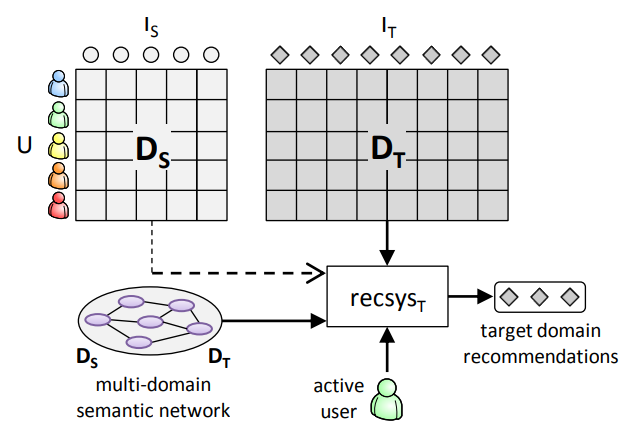
\includegraphics[width=0.8\textwidth]{pictures/linking-domains}
  \caption{Representation of the \textit{linking domains} approach. Source: https://doi.org/10.1007/978-1-4899-7637-6\_27}
\end{figure}
\item \textbf{\textit{Sharing latent features}}: source and target domains are linked by common latent features, such as extracted item features. This approach is similar to the previous one, although it assumes that using denser representations of user preferences or item attributes, which are usually both very sparse sets, leads to more accurate matches. These new representations are obtained with various factorization algorithms. As for the previous approach, at least a feature overlap is strictly needed.
\begin{figure}[hbt!]
  \centering
  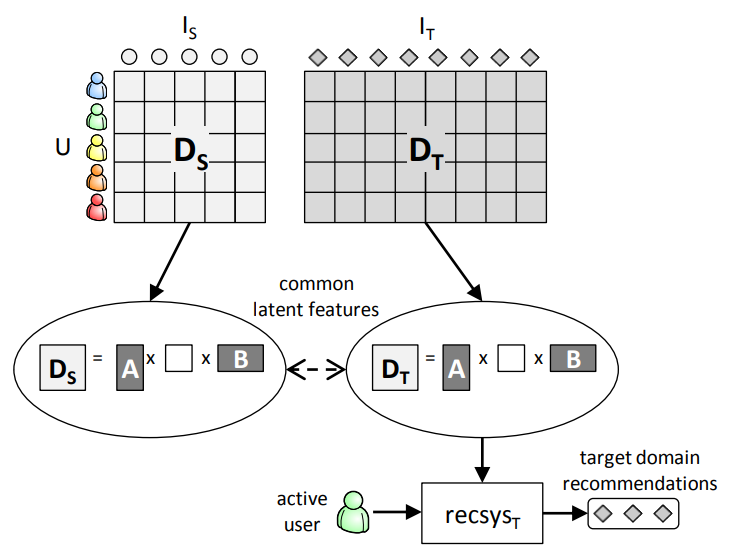
\includegraphics[width=0.8\textwidth]{pictures/sharing-latent-features}
  \caption{Representation of the \textit{sharing latent features} approach. Source: https://doi.org/10.1007/978-1-4899-7637-6\_27}
\end{figure}
\item \textbf{\textit{Transferring rating patterns}}: the rating pattern extracted from one or more source domains is transferred and applied in the target domain.
\begin{figure}[hbt!]
  \centering
  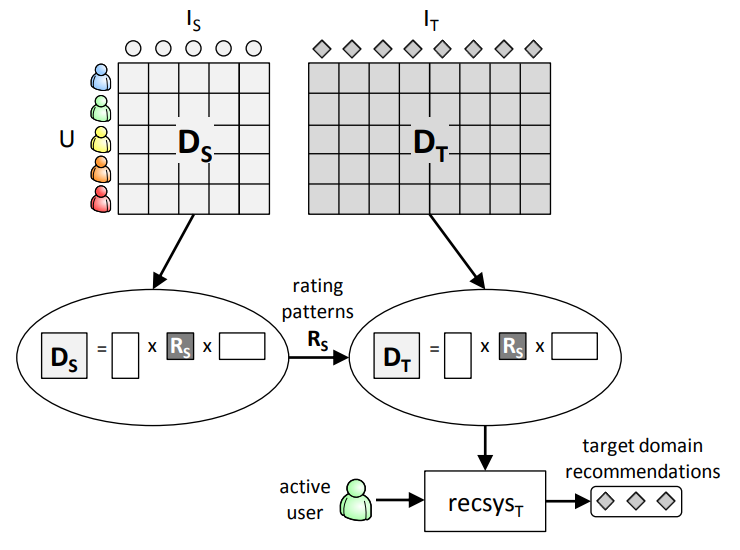
\includegraphics[width=0.8\textwidth]{pictures/transferring-rating-patterns}
  \caption{Representation of the \textit{transferring rating patterns} approach. Source: https://doi.org/10.1007/978-1-4899-7637-6\_27}
\end{figure}
\end{itemize}
\end{itemize}

\begin{figure}[hbt!]
  \centering
  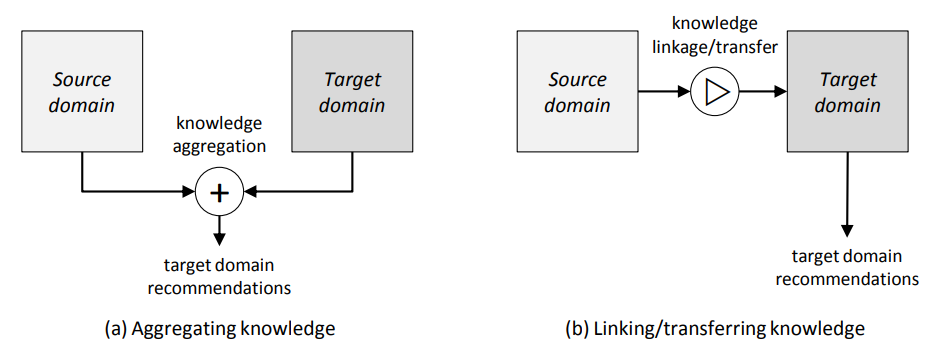
\includegraphics[width=\textwidth]{pictures/knowledge-exploitation}
  \caption{Types of knowledge exploitation in cross-domain recommender systems. Source: https://doi.org/10.1007/978-1-4899-7637-6\_27}
\end{figure}

Since in this thesis we evaluate the codebook transfer technique, we will focus on transferring knowledge and, in particular, on transferring rating patterns.